\begin{figure}
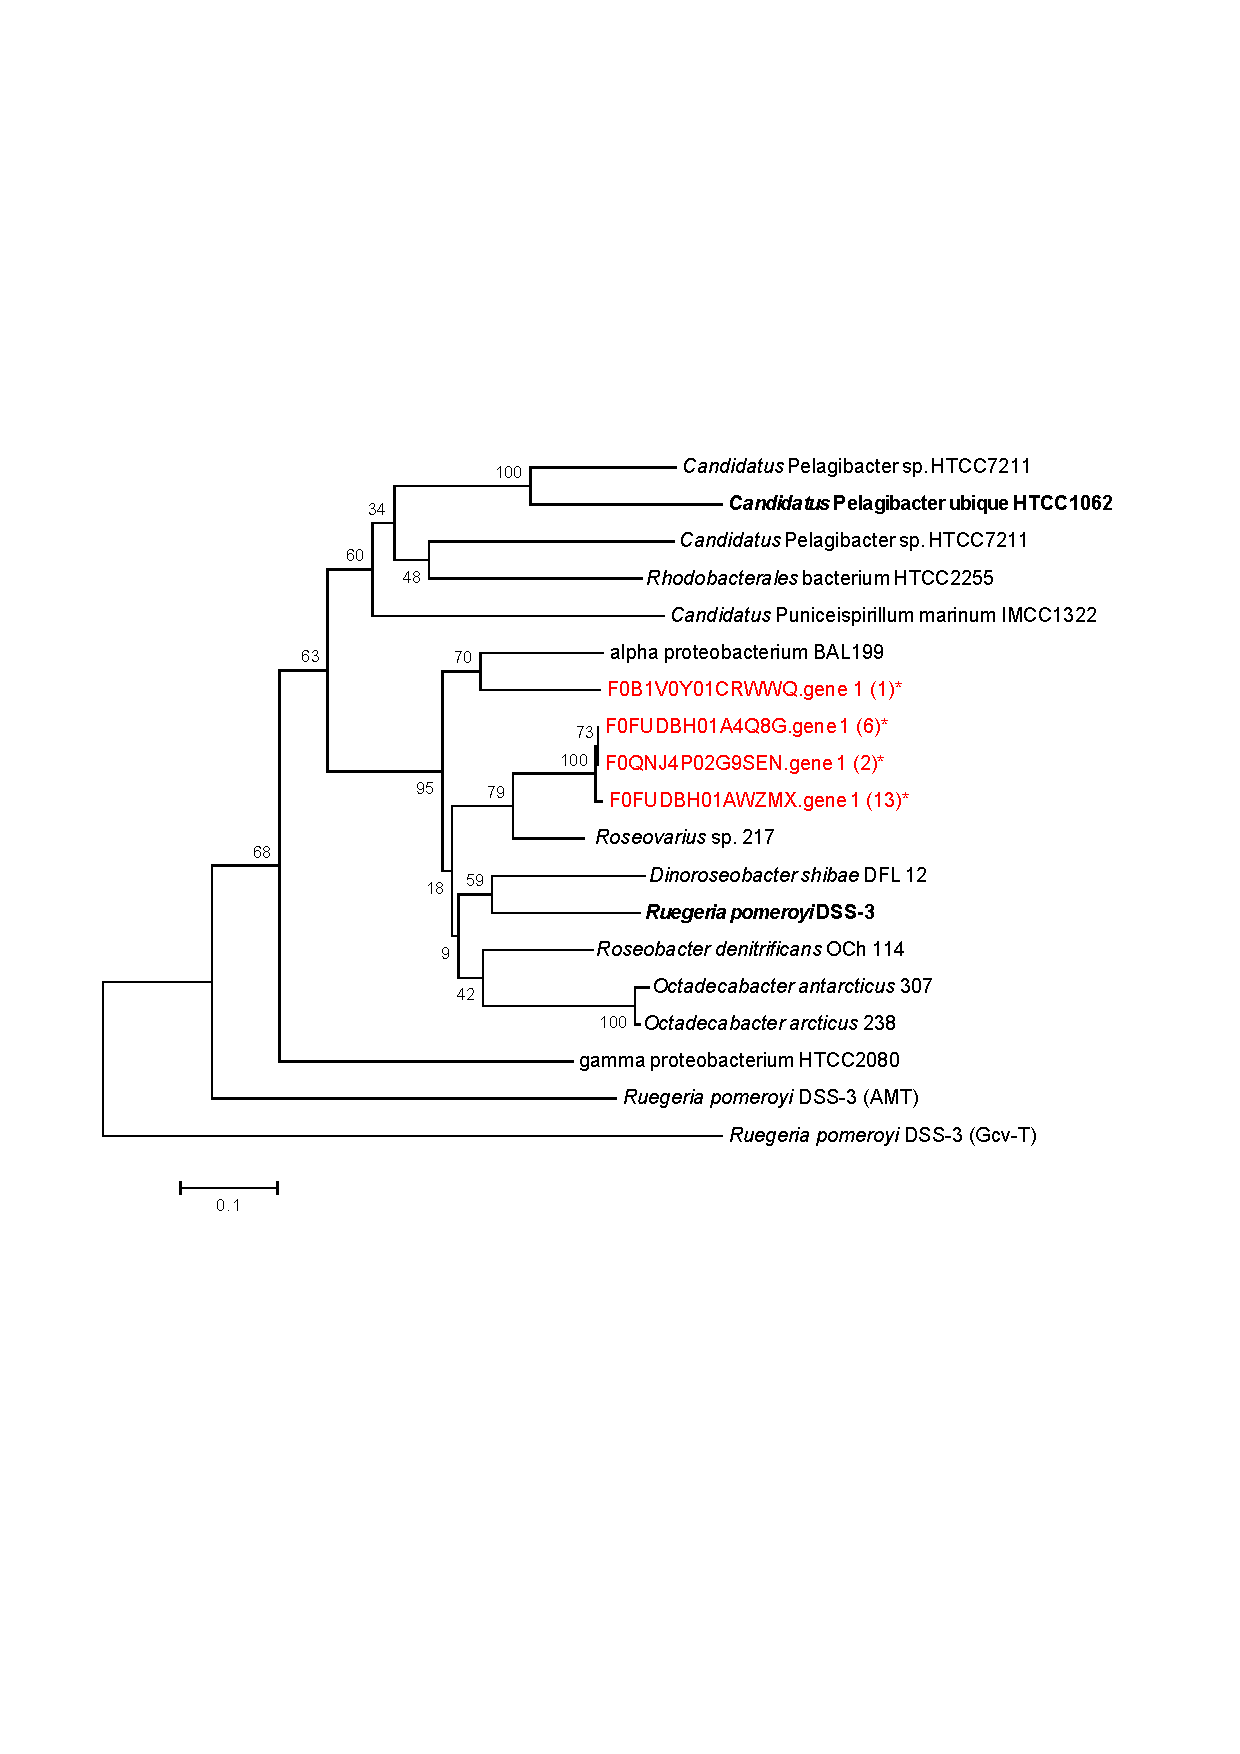
\includegraphics[width=\textwidth]{orglake_figures/dmdA_tree.pdf}
\caption[Phylogenetic tree of DmdA DMSP demethylase homologues]{Phylogenetic tree of DmdA DMSP demethylase homologues. The tree was computed from a 128 amino acid region using the neighbour-joining algorithm. Organic Lake sequences from this study are shown in red and marked with an asterisk (*). Numbers in parentheses are counts of sequences that clustered with the Organic Lake homologue shown in the tree with 90\% amino acid identity. Sequences with confirmed DMSP demethylase activity are shown in bold. Accession numbers from top to bottom are: EDZ60447, YP\_265671, EDZ61098, EAU51039, YP\_003550401, EDP61332, EAQ26389, ABV94056, AAV94935, AAV95190, EDY79173, EDY89914, EAW42451, AAV94935 and AAV97197.}
\label{fig:dmdA_tree}

\end{figure}
